
\newcommand{\medianFKStart}{11.9}
\newcommand{\medianFKEnd}{13.2}
{\bf Readability.}
\label{sec:readability}
Several studies have shown that privacy policies are difficult to read~\cite{mcdonald2008cost,fabian2017large,milne2006longitudinal,li2012online}. 
Here we examine how readability has changed over time.
\begin{figure}
\centering
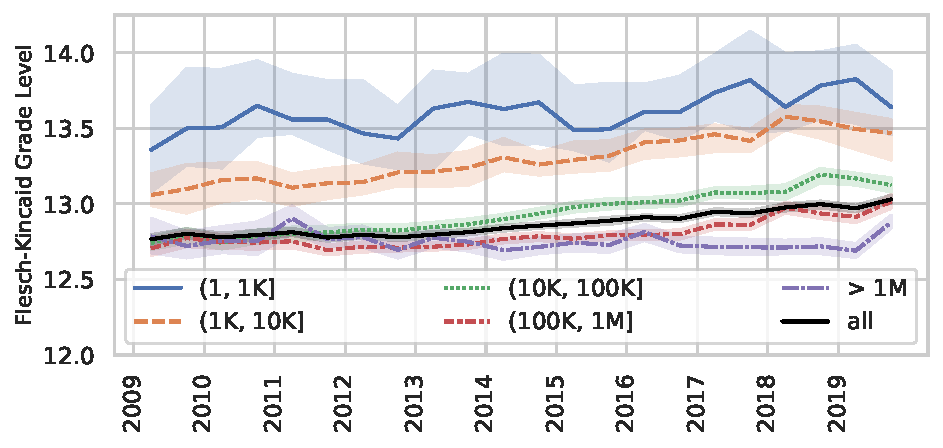
\includegraphics[width=1\columnwidth]{figures/flesch_kincaid_dist.pdf}
\caption{Median Flesch-Kincaid grade level from 2009 to 2019, binned by Alexa rank. 
}
\label{fig:readability}
\end{figure}
We measured readability with the Flesch-Kincaid grade level (FKGL)~\cite{kincaid1975derivation}
using the \textit{py-readability-metrics} Python library~\cite{pyreadabilitymetrics}.
Our preprocessing involved removing non-sentence text such as headers, tables, and lists by writing a custom Markdown renderer using the \emph{Mistune}~\cite{mistune} Python library.

The FKGL measurements are shown in Figure~\ref{fig:readability}. The median readability score has risen more than a grade level from 2000A (\medianFKStart) to 2019B (\medianFKEnd). More popular websites have less readable policies.

In comparison, Li et al.~\cite{li2012online} measured the reading difficulty of privacy policies for websites for the 30 Dow Jones companies in 2012, finding an average FKGL of 13.33, which is similar to our findings for top 1K and top 10K websites.
